\section{Development Results}
\subsection{Segmentation diagnostic}
Over all 997 development items per direction, sentence splitting changes mean COMET by +0.351 for English-to-Tagalog, +0.053 for Tagalog-to-English, +0.292 for English-to-Spanish, and +0.142 for Spanish-to-English. The Tagalog-to-English interval, [-0.019, +0.130], includes zero. The approved split baseline remains primary; these baseline segmentation changes are separate from post-editing gains.

\begin{table}[t]\centering\small
\caption{Sentence-split baseline on the 100-ID development pilot. These are not the full 997-item development scores.}\label{tab:pilotbase}
\begin{tabular}{lrrr}\toprule Direction & BLEU & chrF++ & COMET \\\midrule
En$\to$Tl & 35.884 & 60.632 & 84.442 \\
Tl$\to$En & 46.957 & 67.821 & 87.118 \\
En$\to$Es & 27.694 & 54.086 & 86.076 \\
Es$\to$En & 29.780 & 58.116 & 87.829 \\
\bottomrule\end{tabular}\end{table}

Table~\ref{tab:pilotbase} gives the baseline on the actual 100-ID pilot. Table~\ref{tab:pilot} reports every post-editing condition, retaining all planned items and failures. The sample differs from the full 997-item baseline population.
\begin{table*}[t]
\centering\small
\caption{Development pilot results. Each row uses all 100 planned items, including fallback. COMET (C) and differences ($\Delta$) are reported on the native $\times100$ scale. Intervals are descriptive paired 95\% development intervals; no main-experiment significance is claimed. Zero/One/Reason denote zero-shot, retrieved one-shot, and reason-then-edit.}
\label{tab:pilot}
\begin{tabular}{llrrrrrr}
\toprule
Direction & Strategy & BLEU & chrF++ & C & $\Delta$C & 95\% dev interval & Fallback \\
\midrule
\multicolumn{8}{l}{\textbf{GPT-4o Mini}}\\
En$\to$Tl & Zero & 36.910 & 61.240 & 85.203 & +0.761 & [+0.147, +1.608] & 0 \\
En$\to$Tl & One & 37.757 & 62.087 & 85.905 & +1.463 & [+0.710, +2.396] & 0 \\
En$\to$Tl & Reason & 36.052 & 60.822 & 84.698 & +0.255 & [-0.726, +1.259] & 3 \\
Tl$\to$En & Zero & 47.144 & 68.470 & 87.988 & +0.870 & [+0.396, +1.425] & 0 \\
Tl$\to$En & One & 46.989 & 68.790 & 88.158 & +1.039 & [+0.471, +1.662] & 0 \\
Tl$\to$En & Reason & 47.408 & 68.467 & 87.736 & +0.617 & [+0.154, +1.169] & 4 \\
En$\to$Es & Zero & 28.672 & 54.627 & 86.741 & +0.664 & [+0.238, +1.216] & 0 \\
En$\to$Es & One & 28.260 & 54.475 & 86.695 & +0.619 & [-0.077, +1.295] & 0 \\
En$\to$Es & Reason & 27.946 & 54.180 & 86.077 & +0.001 & [-0.251, +0.298] & 1 \\
Es$\to$En & Zero & 30.297 & 58.418 & 87.846 & +0.018 & [-0.182, +0.194] & 0 \\
Es$\to$En & One & 29.821 & 58.671 & 88.131 & +0.303 & [-0.048, +0.698] & 0 \\
Es$\to$En & Reason & 29.486 & 57.846 & 87.601 & -0.228 & [-0.591, +0.084] & 0 \\
\midrule
\multicolumn{8}{l}{\textbf{Llama 3 8B Instruct}}\\
En$\to$Tl & Zero & 34.201 & 58.363 & 84.348 & -0.094 & [-1.158, +1.071] & 0 \\
En$\to$Tl & One & 33.799 & 59.280 & 84.529 & +0.087 & [-0.997, +1.303] & 0 \\
En$\to$Tl & Reason & 34.222 & 59.139 & 83.806 & -0.637 & [-1.405, +0.389] & 39 \\
Tl$\to$En & Zero & 45.269 & 66.959 & 87.131 & +0.013 & [-0.456, +0.500] & 0 \\
Tl$\to$En & One & 45.659 & 66.896 & 87.471 & +0.352 & [-0.115, +0.932] & 0 \\
Tl$\to$En & Reason & 45.224 & 66.686 & 86.574 & -0.544 & [-0.959, -0.217] & 62 \\
En$\to$Es & Zero & 27.125 & 53.821 & 86.431 & +0.355 & [-0.037, +0.797] & 0 \\
En$\to$Es & One & 27.381 & 53.815 & 86.527 & +0.450 & [-0.050, +0.979] & 0 \\
En$\to$Es & Reason & 26.558 & 53.267 & 85.864 & -0.212 & [-0.570, +0.153] & 65 \\
Es$\to$En & Zero & 29.776 & 57.955 & 87.636 & -0.192 & [-0.553, +0.128] & 0 \\
Es$\to$En & One & 29.942 & 57.590 & 87.783 & -0.046 & [-0.476, +0.384] & 0 \\
Es$\to$En & Reason & 29.202 & 57.240 & 87.267 & -0.562 & [-1.025, -0.192] & 61 \\
\bottomrule
\end{tabular}
\end{table*}


\subsection{Quality changes}
GPT retrieved one-shot has the largest English-to-Tagalog point estimate: +1.463 COMET points, with descriptive interval [0.710, 2.396]. Both Tagalog directions have positive GPT zero-shot and one-shot point estimates. For Spanish-to-English, all three GPT intervals include zero. This evidence does not establish a general low-resource advantage: baseline quality, translation direction, and language pair are confounded.

Llama one-shot estimates are +0.087, +0.352, +0.450, and -0.046 points in the four directions ordered as English-to-Tagalog, Tagalog-to-English, English-to-Spanish, and Spanish-to-English. All four intervals include zero. Reason-then-edit has negative Llama point estimates in every direction. Its intervals exclude zero for the two into-English directions, but remain exploratory. These effects describe the complete operational condition; they do not isolate reasoning from contract compliance.

\subsection{Validity and failure behavior}
All 800 zero-shot/one-shot responses from each model are usable. In reason-then-edit, only 173/400 Llama responses pass the contract, versus 392/400 GPT responses. Thus Llama uses baseline fallback on 227/400 outcomes (56.75\%) and GPT on 8/400 (2\%). Parsing alone is less informative: 399/400 Llama diagnostic responses parse as JSON.

Llama failures include repeated categories (184), invalid note length or emptiness (45), \texttt{NONE} combined with another category (23), diagnostic-count violations (3), and one unparseable, abnormally finished response. These screens overlap and must not be summed. GPT's eight failures all repeat a category. A separate GPT \texttt{NONE} response changes only hyphen spacing; it is disclosed as an instruction-consistency flag and is not retroactively reclassified.

\subsection{Editing and protected drafts}
\begin{table}[t]\centering\footnotesize
\caption{Pooled descriptive pilot counts per 400 outcomes. E: text edited; I/H: metric improvement/harm; P: protect-pool over-edits divided by all 116 protect observations.}\label{tab:harm}
\begin{tabular}{llrrrr}\toprule Editor & Strategy & E & I & H & P \\\midrule
GPT & Zero & 143 & 38 & 8 & 3/116 \\
GPT & One & 320 & 67 & 19 & 6/116 \\
GPT & Reason & 97 & 26 & 20 & 3/116 \\
Llama & Zero & 260 & 37 & 32 & 9/116 \\
Llama & One & 326 & 49 & 37 & 11/116 \\
Llama & Reason & 158 & 8 & 48 & 16/116 \\
\bottomrule\end{tabular}\end{table}

Table~\ref{tab:harm} pools directions descriptively, with 400 outcomes per condition. Retrieved one-shot edits more often than zero-shot for both models. GPT one-shot yields more metric improvements but also more metric harms than GPT zero-shot. Low Llama reason-then-edit activity cannot be called successful restraint because most outputs use fallback. The protect denominator is 116 observations per strategy, with direction-specific counts 22, 45, 21, and 28. Only three Spanish-to-English items fall in the improve pool, limiting subgroup interpretation.

\begin{figure*}[t]
\centering
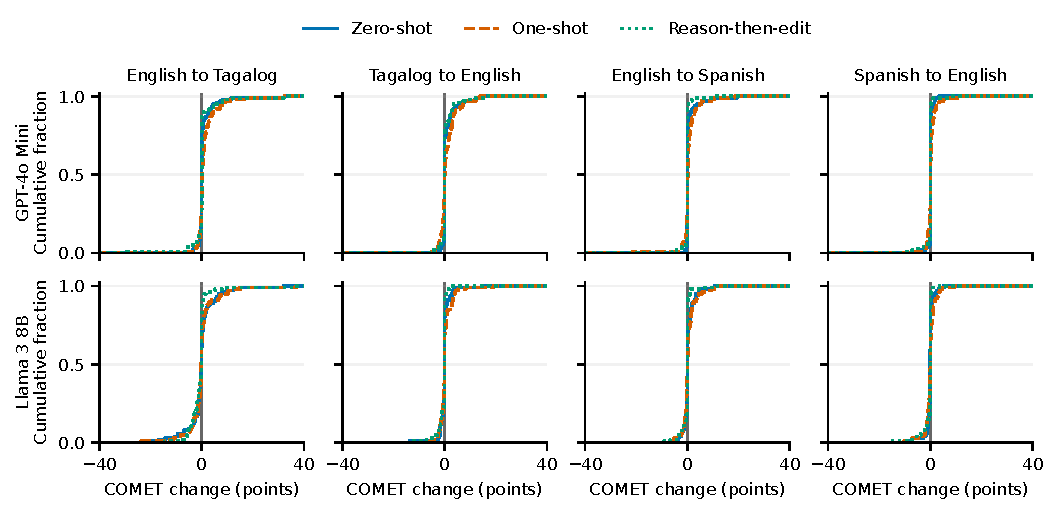
\includegraphics[width=\textwidth]{figures/pilot_delta_ecdf.pdf}
\caption{Empirical distributions of development COMET changes, including every planned outcome. Each curve contains 100 items. The shared point scale retains all observations. Jumps at zero include unchanged translations and baseline fallback; especially for Llama reason-then-edit, that mass must not be interpreted as successful restraint.}
\label{fig:pilotcdf}
\end{figure*}
Figure~\ref{fig:pilotcdf} complements mean differences by retaining the discrete mass at zero and the distribution tails. The curves are descriptive; no pooled independence assumption or stochastic-dominance test is implied.

\subsection{Audit and resource accounting}
The review independently reproduced all BLEU/chrF++ values from raw text, COMET means and paired intervals from aligned numeric caches, raw-record hashes, fallback decisions, and retrieval selections. Neural COMET inference was not rerun during this review. The supplied evaluator rechecked all 400 pilot baselines; the maximum difference was $5.96\times10^{-7}$ native, below the $10^{-5}$ tolerance.

GPT used 643,126 input and 53,095 output tokens with no recorded retries. Applying the recorded uncached token rates gives an estimated charge of approximately \$0.13, not an invoice. Six server fingerprint values occurred within the dated snapshot. Llama's 78 unique generation batches sum to 249.83 seconds of logged wall time, including reused smoke records; initialization is separate. GPT request wall time and Llama batch-amortized time are not comparable per-item speed measurements.
